\documentclass[11pt,a4paper]{article}

\usepackage[T1]{fontenc}
\usepackage[utf8]{inputenc}
\usepackage{lmodern}
\usepackage{microtype}
\usepackage[margin=1in]{geometry}
\usepackage{setspace}
\usepackage{titlesec}
\usepackage{booktabs}
\usepackage{tabularx}
\usepackage{longtable}
\usepackage{array}
\usepackage{multirow}
\usepackage{graphicx}
\usepackage{tikz}
\usetikzlibrary{arrows.meta,calc,positioning}
\usepackage{enumitem}
\usepackage{amsmath}
\usepackage{xcolor}
\usepackage[hyphens]{url}
\usepackage[colorlinks=true,linkcolor=black,citecolor=black,urlcolor=blue]{hyperref}

\onehalfspacing
\setlist[itemize]{leftmargin=1.4em,itemsep=0.2em,topsep=0.3em}
\titleformat{\section}{\large\bfseries}{\thesection}{0.8em}{}
\titleformat{\subsection}{\normalsize\bfseries}{\thesubsection}{0.8em}{}
\titlespacing*{\section}{0pt}{1.4em}{0.6em}
\titlespacing*{\subsection}{0pt}{1.0em}{0.4em}

\begin{document}

\begin{center}
{\LARGE\bfseries Computer Vision for Pediatric Pneumonia\\[0.25em]
Classification from Chest X-rays:\\[0.35em]
A Phase-1 Literature Review}\\[1.1em]
Kartik Yadav \quad Gangadhar Yadav \quad Sahil Sarawgi\\[0.4em]
{\small Semester 7 $\cdot$ Computer Vision Project}\\[0.15em]
{\small August 31, 2026}
\end{center}

\vspace{0.6em}
\noindent\textbf{Abstract---}
This review examines a focused corpus of ten primary studies selected to represent the main methodological stages of computer-vision-based pediatric pneumonia classification: frozen transfer learning, lung-region localization and explainability, from-scratch convolutional networks, multi-task ImageNet transfer, honest radiology-journal evaluation, ensembles that expose the viral class, external-hospital testing, hybrid CNN--transformers with synthetic minority data, and lightweight freeze-versus-fine-tune comparisons. The Guangzhou Women and Children's Medical Center collection released by Kermany et al.\ is the recurring benchmark, but several studies quietly replace the official 624-patient test, and one takes the same pipeline off-site. Across the literature, strong binary accuracy on curated Guangzhou films is common, while the harder problems are consistent evaluation, three-class and bacterial-versus-viral labels, class imbalance, and domain shift. The review therefore treats reported accuracy as task- and split-dependent rather than as a direct ranking of models. Four candidate research gaps are identified, with consistent evaluation on the official 624-patient test, together with the viral class, emerging as the strongest and most feasible gap for a student reproduction study.

\vspace{0.4em}
\noindent\textit{Index terms---}pediatric pneumonia, chest X-ray, Kermany dataset, Guangzhou Women and Children's Medical Center, convolutional neural networks, transfer learning, class imbalance, explainable AI.

\tableofcontents
\newpage

\section{Introduction}
Pediatric pneumonia is a natural application for computer vision because the diagnostic evidence is visual, but the task is difficult. The film is a frontal chest radiograph of a child aged one to five. Bacterial disease tends to present as focal lobar consolidation; viral disease as a more diffuse interstitial pattern; a normal film as clear lungs~\cite{kermany2018}. The decision is not academic. Bacterial pneumonia wants antibiotics; viral pneumonia wants supportive care; a normal film wants observation. A binary ``pneumonia'' score cannot tell a clinician which of those three rooms to send the child to.

Kermany et al.\ made this problem public~\cite{kermany2018}. Their \textit{Cell} paper is mostly about retinal OCT. The chest X-rays are the generalization experiment, and that experiment became the default exam. About 5{,}856 frontal films from Guangzhou Women and Children's Medical Center, later mirrored on Kaggle as Chest X-Ray Images (Pneumonia). Every later paper in this review is arguing with that set, even when the authors appear to be arguing with a backbone.

The literature considered here is deliberately focused. Ten primary studies, 2018--2026, all read in full (local PDF, arXiv, or open PMC/MDPI), together illustrate the field's movement from a frozen ImageNet classifier toward localization, three-task reporting, ensembles, external testing, hybrids, and tiny nets. Extra ImageNet ensembles that only reprint a binary score were left out. One additional paper is used only as supporting context for off-site drop~\cite{xin2021}.

The main question for Phase~1 is therefore not which model reports the highest accuracy, but: how has the problem formulation and methodology evolved, what weaknesses repeatedly appear in the evidence, and which unresolved problems are realistic research directions?

\section{Review Scope and Corpus}
The ten-paper core is the set identified in the accompanying survey notes. It includes the dataset-defining \textit{Cell} paper~\cite{kermany2018}, the first strong localization study~\cite{rajaraman2018}, a from-scratch CNN~\cite{stephen2019}, the first side-by-side three-task transfer study~\cite{rahman2020}, an honest radiology-journal report~\cite{salehi2021}, two ensemble papers that surface the viral class and an external hospital~\cite{ayan2021,kundu2021}, a hybrid CNN--transformer with GAN minority synthesis~\cite{raghaw2024}, a 388k-parameter net~\cite{chauhan2025}, and a controlled freeze-versus-fine-tune comparison~\cite{choudhury2026}.

The analysis below uses the papers as the primary evidence base. Where a paper's publicly verifiable material does not expose a split, a metric, or a preprocessing step, this review does not invent it. Headline metrics are accuracy, sensitivity/recall, specificity, F1, and AUC. The split is treated as part of the result, not as a footnote.

\section{The Kermany Benchmark and the Problem Formulation}
The Guangzhou collection became a benchmark because it is public, labeled, and small enough to train on a single GPU. Kermany et al.\ report two tasks, not one~\cite{kermany2018}. Pneumonia versus normal: accuracy 92.8\%, sensitivity 93.2\%, specificity 90.1\%, AUC 96.8\%. Bacterial versus viral: accuracy 90.7\%, sensitivity 88.6\%, specificity 90.9\%, AUC 94.0\%. The etiology call is already worse. That gap is the start of the timeline, not a later discovery.

Two facts from the source PDF keep getting smeared in later tables. First, they \emph{froze} Inception~V3 and trained only the softmax; unfreezing the convolutional stack decreased accuracy through overfitting. Second, pneumonia-versus-normal specificity is 90.1\%, not precision. Rahman et al.\ quote that number as precision in their comparison table~\cite{rahman2020}. The \textit{Cell} text says specificity.

The split, from the paper, not from Kaggle: 5{,}232 train images (1{,}349 normal, 2{,}538 bacterial, 1{,}345 viral) and a patient-independent test of 624 patients (234 normal, 242 bacterial, 148 viral). Kaggle later peels 16 training images into a toy validation folder. That folder is not in the \textit{Cell} protocol. Papers that keep the 624 test and papers that carve 80/10/10 from train are sitting different exams. They should not be ranked on one board.

The benchmark is useful because it makes reproduction possible. It is also narrower than the clinic. One hospital, ages 1--5, frontal films only, pneumonia outnumbering normal about 3:1, bacterial outnumbering viral. Salehi et al.\ warn that same-patient images may leak across splits~\cite{salehi2021}. Kundu et al.\ take a 98.8\% Kermany model to RSNA and land at 87\%~\cite{kundu2021}. Xin et al.\ likewise report limited generalizability of a pediatric pneumonia classifier on external radiographs~\cite{xin2021}. Those sentences are the limit of what a Guangzhou JPEG can prove.

\begin{figure}[t]
\centering
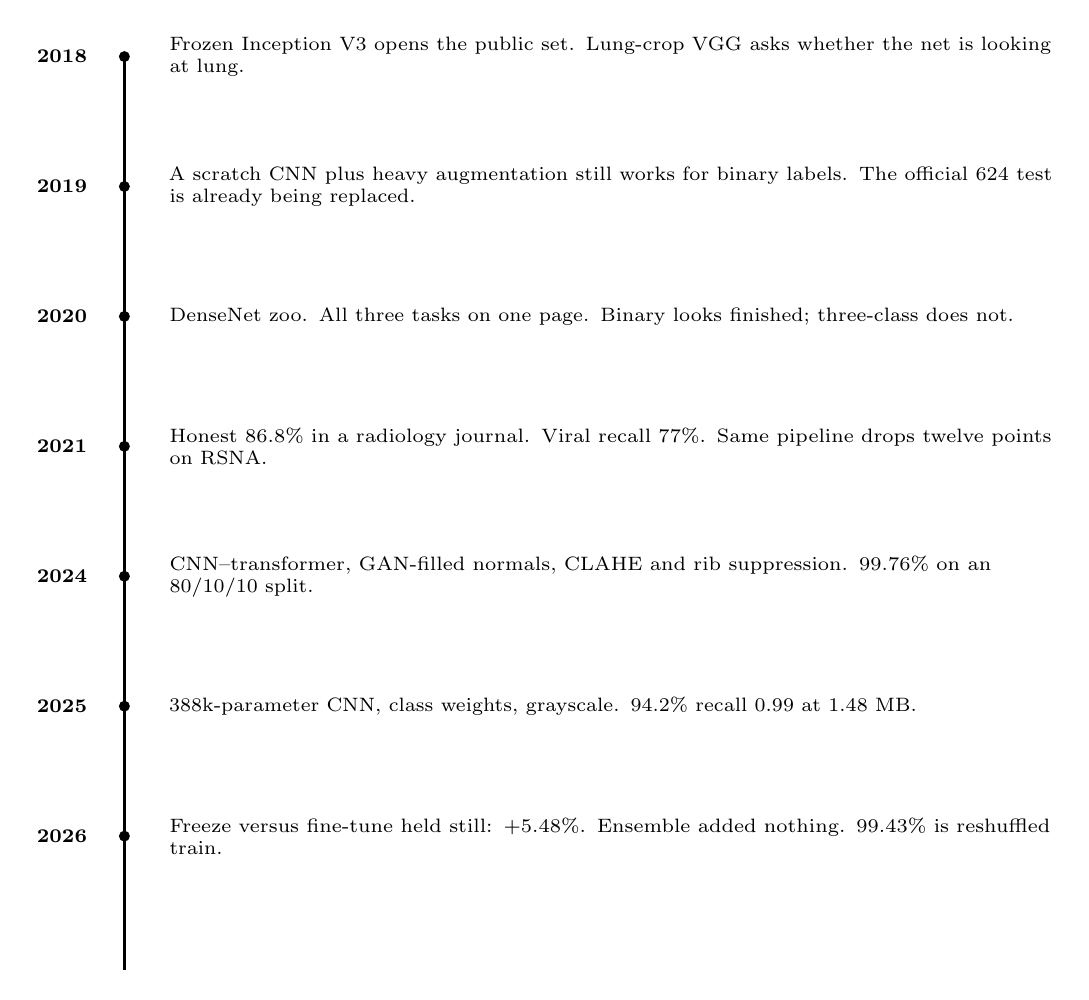
\begin{tikzpicture}[
  year/.style={font=\scriptsize\bfseries, anchor=east},
  ev/.style={font=\scriptsize, align=left, text width=11.2cm, anchor=west},
  dot/.style={circle, fill=black, inner sep=1.4pt}
]
\draw[line width=1.15pt] (0,0) -- (0,-11.6);
\foreach \y/\yr/\txt in {
  0/2018/{Frozen Inception~V3 opens the public set. Lung-crop VGG asks whether the net is looking at lung.},
  -1.65/2019/{A scratch CNN plus heavy augmentation still works for binary labels. The official 624 test is already being replaced.},
  -3.3/2020/{DenseNet zoo. All three tasks on one page. Binary looks finished; three-class does not.},
  -4.95/2021/{Honest 86.8\% in a radiology journal. Viral recall 77\%. Same pipeline drops twelve points on RSNA.},
  -6.6/2024/{CNN--transformer, GAN-filled normals, CLAHE and rib suppression. 99.76\% on an 80/10/10 split.},
  -8.25/2025/{388k-parameter CNN, class weights, grayscale. 94.2\% recall 0.99 at 1.48~MB.},
  -9.9/2026/{Freeze versus fine-tune held still: +5.48\%. Ensemble added nothing. 99.43\% is reshuffled train.}
} {
  \node[dot] at (0,\y) {};
  \node[year] at (-0.35,\y) {\yr};
  \node[ev] at (0.45,\y) {\txt};
}
\end{tikzpicture}
\caption{Timeline of the ten-paper corpus. The field did not merely swap backbones. It changed what it asked the system to do, and, just as often, quietly changed the exam.}
\label{fig:timeline}
\end{figure}

\section{Evolution of Methods}
\label{sec:evolution}
Figure~\ref{fig:timeline} is the spine of this review. The subsections below follow that spine as a sequence of methodological stages, not as a leaderboard of architectures.

\subsection{Frozen transfer learning opens the set}
Kermany et al.\ took ImageNet-pretrained Inception~V3, froze the convolutional layers, cached bottleneck activations, and trained a softmax~\cite{kermany2018}. Adam, learning rate 0.001, 100 epochs, a GTX~1080. Low-quality and unreadable films were removed. No geometric augmentation, no class weights, no lung crop. The clinical mapping---urgent referral, supportive care, observation---is in the paper. The CXR experiment itself is a generalization paragraph plus Figure~6, not a full methods paper: no CXR confusion matrix, no joint three-class accuracy, no viral recall, no CXR occlusion map.

That is still the opening move of the whole literature. Transfer learning made a 5{,}800-image pediatric set trainable. The freeze decision is the 2018 answer. A 2026 paper on the same JPEGs will say the opposite~\cite{choudhury2026}. The disagreement is now an experiment.

\subsection{Localization: whether the net is looking at lung}
Six months later Rajaraman et al.\ cut the last VGG16 layer, put global average pooling and a dense head on top, and cropped to lungs with an anatomical-atlas detector~\cite{rajaraman2018}. Whole film and crop both resampled to $1024\times 1024$, mean-normalized. Noisy images stayed in training ``to reduce bias and overfitting.'' Customized VGG16 beat sequential, residual, and Inception variants on this small, low-variance pediatric set.

On the cropped ROI: pneumonia versus normal, accuracy 96.2\%, AUC 0.993; bacterial versus viral, accuracy 93.6\%, specificity 0.86. Average-CAM and LIME. Cropping beat the full film. The atlas detector under-segments costophrenic angles. The methodological change is not a higher number. It is the question: localization, not just a score. Saliency maps show where a prediction is associated with image evidence. They do not prove that the reasoning is medically valid.

\subsection{From-scratch convolutional networks}
Stephen et al.\ trained a small convolutional net from scratch---conv, max-pool, ReLU, dropout, dense, sigmoid---and used aggressive Keras augmentation instead of ImageNet weights~\cite{stephen2019}. Best size $200\times 200\times 3$. Training accuracy 95.31\%, validation accuracy 93.73\%. Binary only. They reshuffled into 3{,}722 train / 2{,}134 validation. That is not the official 624.

The sentence this paper contributes is simple. ImageNet is not required for a binary Kermany label. A custom split also cannot be ranked against Kermany's test. Both things are true at once.

\subsection{The ImageNet zoo, and all three tasks on one page}
Rahman et al.\ ran AlexNet, ResNet18, DenseNet201, and SqueezeNet, and put binary, three-class, and bacterial-versus-viral results side by side~\cite{rahman2020}. DenseNet201 wins all three. Geometric augmentation until each class has 4{,}500 training images. Their own test, about 200 images per class, not the 624.

DenseNet201: normal versus pneumonia 98.0\% accuracy; three-class 93.3\%; bacterial versus viral 95.0\%. Confusion matrices show bacterial and viral swapping. Binary looks better than three-class because the easy split is doing the work. This is the first paper in the corpus that makes that comparison unavoidable. It is also the paper that mislabels Kermany's 90.1\% specificity as precision.

\subsection{Honest numbers, ensembles, and the viral class}
Three papers in 2021 change the argument.

Salehi et al., in the \textit{British Journal of Radiology}, report DenseNet121 at 86.8\% accuracy and AUC 0.86, with SMOTE, after a string of 98s~\cite{salehi2021}. Sensitivity stays above 91\%. They warn that same-patient leakage likely inflates published accuracy, and that laterals---needed in about 15\% of real reads---are absent.

Ayan, Karabulut and \"Unver ensemble three nets, not seven (bigger ensembles got worse), and publish the number this project actually has to live with: viral recall 77.03\% against bacterial recall 97.93\%; three-class ensemble accuracy 90.71\%~\cite{ayan2021}. They augmented 1{,}349 normals up to 2{,}534. The 624 test looks official. Viral pneumonia will not sit still.

Kundu et al.\ train a weighted ensemble of GoogLeNet, ResNet-18 and DenseNet-121, post 98.81\% on Kermany, and then run the same pipeline on RSNA: 86.95\%~\cite{kundu2021}. Twelve points. Weighted average, not majority vote. After this paper, ``can a CNN beat 90\% on Guangzhou children?'' is the wrong question.

\subsection{Hybrids, synthetic minority, and a different exam}
XCCNet (Raghaw, Bhore, Rehman and Kumar) fuses a dilated spatial CNN with a contrastive transformer, fills the normal class with GAN-style images (1{,}583 $\rightarrow$ 4{,}207), and runs a heavy preprocess stack: CLAHE, lung segmentation, rib suppression~\cite{raghaw2024}. Headline accuracy 99.76\%. Ablation: no augmentation 96.29\%; traditional augmentation 97.18\%; full stack 99.76\%. Also evaluated on VinDr-PCXR, NIH-Pediatric, and Trivedi. Grad-CAM, Score-CAM, LIME.

The split is 80/10/10, balanced, heavily preprocessed. Not the official 624. The 99.76\% is evidence that the stack works under that protocol. It is not a successor to Kermany's 92.8\%.

\subsection{Efficiency, and freeze versus fine-tune held still}
Chauhan, Gupta and Doja train LightPneumoNet from scratch: 388{,}082 parameters, 1.48~MB, class weights (normal 2.0, pneumonia 1.2), grayscale input, no horizontal flip because left and right anatomy mean something~\cite{chauhan2025}. Official-style independent test: 94.2\% accuracy, precision 0.92, recall 0.99. High recall at a size that fits a lab GPU. Binary. They wrote the precision trade down.

Choudhury finally holds freeze versus fine-tune still~\cite{choudhury2026}. Custom 4-block CNN versus ResNet50, DenseNet121, and EfficientNet-B0, each frozen or fine-tuned on the last two blocks. ResNet50 fine-tune: 99.43\% accuracy, three errors on 523 images. Fine-tune beats frozen by +5.48\% accuracy on average. Ensemble added nothing. They discard the 16-image Kaggle validation folder and carve a stratified 80/10/10 from the 5{,}216 training images. Seed 42. Grad-CAM on TP/TN/FP/FN.

Best controlled ablation in the pile. Also the clearest warning: 99\% is on a reshuffled split, not Kermany's official test. The 2018 freeze that hurt and the 2026 fine-tune that helped have never been run on the same 624-patient exam.

\section{Comparative Analysis of the Selected Literature}
Table~\ref{tab:matrix} compares problem formulation and evidence, not models by a single number. Metrics from different splits, tasks, and hospitals should not be read as a ranking.

{\small
\setlength{\tabcolsep}{3.5pt}
\begin{longtable}{>{\raggedright\arraybackslash}p{0.17\textwidth}
                  >{\raggedright\arraybackslash}p{0.20\textwidth}
                  >{\raggedright\arraybackslash}p{0.18\textwidth}
                  >{\raggedright\arraybackslash}p{0.20\textwidth}
                  >{\raggedright\arraybackslash}p{0.17\textwidth}}
\caption{Selected literature matrix for the ten-paper core corpus.}
\label{tab:matrix}\\
\toprule
\textbf{Study} & \textbf{Data / task} & \textbf{Method} & \textbf{Main contribution} & \textbf{Main limitation or open issue} \\
\midrule
\endfirsthead
\toprule
\textbf{Study} & \textbf{Data / task} & \textbf{Method} & \textbf{Main contribution} & \textbf{Main limitation or open issue} \\
\midrule
\endhead
\bottomrule
\endfoot
Kermany et al.\ (2018) &
Guangzhou CXR; 2 binaries; official 624 &
Frozen Inception~V3 &
Creates the public pediatric set; 92.8\% / 90.7\% &
CXR is a side experiment; freeze later disputed \\
\addlinespace
Rajaraman et al.\ (2018) &
Same set; 2 binaries + 3-class; 624 &
Custom VGG16; lung crop $1024^2$; CAM/LIME &
Shows cropping to lung beats the full film &
Atlas crop under-segments costophrenic angles \\
\addlinespace
Stephen et al.\ (2019) &
Binary; reshuffled 3722/2134 &
Scratch CNN + heavy Keras aug &
Proves ImageNet is not required for binary Kermany &
Custom split; no AUC table; binary only \\
\addlinespace
Rahman et al.\ (2020) &
2 binaries + 3-class; own $\sim$200/class test &
DenseNet201 wins; aug to 4{,}500/class &
First clean three-task comparison; 98.0 / 93.3 / 95.0 &
Not the official 624; Table~5 mislabels Kermany specificity as precision \\
\addlinespace
Salehi et al.\ (2021) &
Binary; radiology journal &
DenseNet121 + SMOTE &
Honest 86.8\%; warns about patient leakage &
Binary; still one hospital \\
\addlinespace
Ayan et al.\ (2021) &
Binary + 3-class; 624-like test &
Ensemble of three CNNs &
Viral recall 77\% vs bacterial 98\% &
Viral class unsolved; trial-and-error hyperparameters \\
\addlinespace
Kundu et al.\ (2021) &
Binary; Kermany then RSNA &
Weighted ensemble of three CNNs &
98.8\% $\rightarrow$ 87\% off-site; first widely cited external drop &
Triple cost; binary; fails on early infiltrates \\
\addlinespace
Raghaw et al.\ (2024) &
Binary; 80/10/10; four datasets &
CNN--transformer; GAN normals; CLAHE/ribs &
99.76\% under a heavy stack; module ablations &
Not the official 624; needs lung/rib labels \\
\addlinespace
Chauhan et al.\ (2025) &
Binary; official-style test &
388k CNN; class weights; grayscale &
94.2\% at 1.48~MB; high recall written down with precision 0.92 &
Binary; small data acknowledged \\
\addlinespace
Choudhury (2026) &
Binary; 80/10/10 of 5{,}216 train &
ResNet50 fine-tune vs freeze vs scratch &
+5.48\% for fine-tune; ensemble added nothing &
99.43\% is reshuffled, not the 624 \\
\end{longtable}
}

\noindent\textit{Note.} The table records the evidence available for the selected studies. A reported 99\% on an 80/10/10 split is not comparable to 92.8\% on the 624-patient \textit{Cell} test.

\section{Cross-Paper Findings}

\subsection{The main shift is in the exam, not only the architecture}
The literature did not progress simply from Inception to VGG to DenseNet to a transformer. The more consequential changes are in what is being asked, and on which split. Early work reports two binaries on the official 624~\cite{kermany2018,rajaraman2018}. Then the exam quietly moves: a reshuffled train/val~\cite{stephen2019}, a private $\sim$200/class test~\cite{rahman2020}, 80/10/10 of train~\cite{raghaw2024,choudhury2026}. Three-class and bacterial-versus-viral are the clinically complete tasks and the ones that drop several points~\cite{rahman2020,ayan2021}. Ranking backbones on mixed exams is not a finding. It is a category error.

\subsection{Kermany accuracy has become a weak standalone indicator}
Binary numbers on this set commonly land between 93\% and 99\%. Salehi's 86.8\%~\cite{salehi2021} and Kundu's 87\% on RSNA~\cite{kundu2021} are the more informative figures. High in-set accuracy is evidence of learnability on Guangzhou JPEGs. It is not evidence that pediatric pneumonia classification is solved.

\subsection{Viral pneumonia is the class that will not sit still}
Kermany already: bacterial-versus-viral 90.7\% / 88.6\% sensitivity against pneumonia-versus-normal 92.8\% / 93.2\%~\cite{kermany2018}. Ayan: viral recall 77\% versus bacterial 98\%~\cite{ayan2021}. Rahman: three-class 93.3\% versus binary 98\%~\cite{rahman2020}. Binary accuracy is inflated by the easy normal-versus-obvious-consolidation split. Three-class accuracy, with per-class viral recall, is the honest headline.

\subsection{CNNs remain the workhorse after the hybrid shift}
The 2024 transformer hybrid does not retire convolutional networks. DenseNet121/201 win Rahman and Salehi~\cite{rahman2020,salehi2021}. ResNet50 wins the 2026 bake-off~\cite{choudhury2026}. A 388k scratch CNN still posts 94.2\% with recall 0.99~\cite{chauhan2025}. The more defensible conclusion is that the field is moving toward a broader design space rather than replacing one family with another.

\subsection{Freeze, crop, and ensemble are still open knobs}
Kermany froze Inception~V3 and said unfreezing hurt~\cite{kermany2018}. Choudhury fine-tuned last blocks and gained 5.48\%, and ensembles added nothing once ResNet50 was fine-tuned~\cite{choudhury2026}. Rajaraman and XCCNet say lung crop helps~\cite{rajaraman2018,raghaw2024}; most notebooks skip it. Ayan and Kundu need three towers~\cite{ayan2021,kundu2021}. None of these knobs have been ablated on one shared, patient-level 624 test.

\subsection{Imbalance is handled with augmentation, almost never with a fancy loss}
Rotate, shift, shear, zoom, flip. Minority oversampling~\cite{ayan2021}. Balance-to-$N$~\cite{rahman2020}. SMOTE~\cite{salehi2021}. Class weights~\cite{chauhan2025}. GAN normals~\cite{raghaw2024}. Focal loss lives in COVID-era four-class papers, not here. Horizontal flip is not free; LightPneumoNet turns it off~\cite{chauhan2025}.

\section{Limitations of the Evidence Base}
\paragraph{Single hospital, single age band.}
Almost the entire corpus trains and tests on Guangzhou children aged 1--5. Kundu's RSNA drop~\cite{kundu2021} and Xin et al.'s external-data result~\cite{xin2021} are the existence proof that this matters, and almost nobody repeats that move.

\paragraph{Evaluation heterogeneity.}
Studies differ in train/test splitting, augmentation, input size, class count, and whether patients can leak. A 99\% binary accuracy on an 80/10/10 split cannot be read as beating 92.8\% on the official 624.

\paragraph{Task substitution.}
Binary normal-versus-pneumonia is publishable and clinically incomplete. Three-class and bacterial-versus-viral numbers sit 4--8 points lower and are reported less often.

\paragraph{Reproducibility details.}
The best-documented studies name the backbone, the split, and the metric. Some later preprints expose only part of the protocol. Where a setting could not be verified, it is not used to support a stronger claim. Rahman et al.'s mislabeling of Kermany specificity as precision is a reminder to go back to the source PDF~\cite{rahman2020,kermany2018}.

\section{Research Gaps}
The gaps below are narrow enough to be useful for a student research-reproduction project.

\subsection{Gap 1 --- Consistent evaluation on the official 624-patient test}
\paragraph{Evidence.}
The \textit{Cell} protocol is 5{,}232 train and a 624-patient held-out test~\cite{kermany2018}. Kaggle is 5{,}216 / 16 / 624. Stephen reshuffles~\cite{stephen2019}. Rahman uses a private test~\cite{rahman2020}. XCCNet and Choudhury carve 80/10/10 from train and report 99\%~\cite{raghaw2024,choudhury2026}. Papers that keep the 624 report 86--95\%.

\paragraph{Why it remains unresolved.}
Cross-paper accuracy comparisons are difficult when the unit of evaluation changes. The 16-image validation folder is still treated as a real split in notebooks. The literature consequently provides evidence for learnability on Guangzhou JPEGs, but mixed evidence for which method is actually better.

\paragraph{Feasibility.}
High. A reproduction can freeze one protocol---the \textit{Cell} 624, or a documented patient-level 80/10/10, never both silently---and rerun two or three backbones against it.

\subsection{Gap 2 --- Three-class labels and the viral minority}
\paragraph{Evidence.}
Kermany's bacterial-versus-viral gap~\cite{kermany2018}; Rahman's three-class drop~\cite{rahman2020}; Ayan's 77\% viral recall~\cite{ayan2021}. Antibiotics depend on this distinction.

\paragraph{Why it remains unresolved.}
Binary screening numbers keep getting published because they look finished. The hard class is still viral pneumonia, and most recent 99\% papers are binary again~\cite{raghaw2024,chauhan2025,choudhury2026}.

\paragraph{Feasibility.}
High. The labels are already in the dataset. The experiment is to report per-class recall, especially viral, on a fixed split.

\subsection{Gap 3 --- Cross-hospital generalization}
\paragraph{Evidence.}
Kundu 98.8\% $\rightarrow$ 87\% on RSNA~\cite{kundu2021}. Xin et al.\ report limited generalizability of a pediatric pneumonia deep-learning system on external radiographs~\cite{xin2021}. Salehi and Choudhury both list single-center pediatric data as the main limitation and then stay inside it~\cite{salehi2021,choudhury2026}.

\paragraph{Why it remains unresolved.}
There is no multi-hospital Kermany-style label protocol. High Guangzhou accuracy and off-site robustness are measured under different conditions.

\paragraph{Feasibility.}
Moderate-to-high. A strong Kermany baseline can be evaluated on a public adult or mixed CXR pneumonia set (RSNA, or a documented subset) without inventing a new architecture.

\subsection{Gap 4 --- Freeze versus fine-tune, and full film versus lung crop, on one split}
\paragraph{Evidence.}
Kermany reports that unfreezing Inception~V3 hurt~\cite{kermany2018}. Choudhury reports that fine-tuning the last blocks of ResNet and DenseNet gained 5.48\%~\cite{choudhury2026}. Rajaraman and XCCNet crop to lung~\cite{rajaraman2018,raghaw2024}.

\paragraph{Why it remains unresolved.}
The two freeze results were never compared on the official 624 with the same preprocess. Crop versus full film is still a notebook opinion.

\paragraph{Feasibility.}
High for freeze/fine-tune on Kermany. Moderate for a clean lung-crop ablation if an off-the-shelf segmenter is used rather than a full annotation pipeline.

\subsection{Gap ranking}
For this semester the strongest candidate is \emph{consistent evaluation on the official 624, with three-class or bacterial-versus-viral as a reported task}, followed by freeze-versus-fine-tune on that same split, then a modest external test. Instance-level detection on whole fields of view is scientifically attractive and out of scope. The ranking is based on recurrence in the ten papers and on what a three-person team can actually run, not on an assumption that these are the only important open problems.

\section{Implications for the Research-Reproduction Project}
A defensible Phase-2 baseline is a well-documented Kermany classifier whose preprocess, trainer, and split can be reproduced from a README. The purpose of that baseline is a trustworthy reference point, not another 99.

The literature suggests the most meaningful single change is one that tests the exam or the hard class rather than swapping a backbone. Concretely: the \textit{Cell} 624-patient test, or a documented patient-level 80/10/10, never both silently; binary \emph{and} bacterial-versus-viral, the two tasks the source paper reports; ResNet50 frozen versus last-block fine-tune versus a small scratch CNN; class weights or minority augmentation; $224\times 224$, ImageNet normalization, modest rotation/shift; per-class viral recall; Grad-CAM on errors, aimed at Figure~S6 of the \textit{Cell} paper (focal consolidation versus interstitial pattern)~\cite{kermany2018}. If a number only exists because train was reshuffled, it gets written next to the number.

\section{Conclusion}
The selected literature shows a clear maturation of pediatric pneumonia computer vision on one public set. The field moved from a frozen Inception~V3, to asking whether the net looked at lung, to scratch CNNs, to an ImageNet zoo with three-task reporting, to honest lower numbers, to ensembles that expose viral failure, to an external-hospital drop, to hybrids and tiny nets and a 99\% that lives on a different split.

The hardest problems did not disappear as accuracy increased. They moved outward: from recognizing obvious consolidation on a Guangzhou JPEG to deciding bacterial versus viral, to keeping the official test, to surviving another hospital's films.

For Phase~1, the central conclusion is that this task should not be evaluated solely by the highest Kermany binary accuracy. The stronger research question is whether the learned representation remains reliable when the class, the split, or the site changes, and whether the evaluation protocol makes that reliability measurable. That is the basis for selecting a reproducible baseline and a research gap for the next phase.

\begin{thebibliography}{11}

\bibitem{kermany2018}
D.~S. Kermany, M.~Goldbaum, W.~Cai \textit{et al.}, ``Identifying medical diagnoses and treatable diseases by image-based deep learning,'' \textit{Cell}, vol.~172, no.~5, pp.~1122--1131.e2, 2018, doi: 10.1016/j.cell.2018.02.010. Data: doi: 10.17632/rscbjbr9sj.3.

\bibitem{rajaraman2018}
S.~Rajaraman, S.~Candemir, I.~Kim, G.~Thoma, and S.~Antani, ``Visualization and interpretation of convolutional neural network predictions in detecting pneumonia in pediatric chest radiographs,'' \textit{Appl.\ Sci.}, vol.~8, no.~10, p.~1715, 2018, doi: 10.3390/app8101715.

\bibitem{stephen2019}
O.~Stephen, M.~Sain, U.~J. Maduh, and D.-U. Jeong, ``An efficient deep learning approach to pneumonia classification in healthcare,'' \textit{J.\ Healthc.\ Eng.}, vol.~2019, p.~4180949, 2019, doi: 10.1155/2019/4180949.

\bibitem{rahman2020}
T.~Rahman, M.~E.~H. Chowdhury \textit{et al.}, ``Transfer learning with deep convolutional neural network (CNN) for pneumonia detection using chest X-ray,'' arXiv:2004.06578, 2020.

\bibitem{salehi2021}
M.~Salehi, R.~Mohammadi, H.~Ghaffari, N.~Sadighi, and R.~Reiazi, ``Automated detection of pneumonia cases using deep transfer learning with paediatric chest X-ray images,'' \textit{Br.\ J.\ Radiol.}, vol.~94, p.~20201263, 2021, doi: 10.1259/bjr.20201263.

\bibitem{ayan2021}
E.~Ayan, B.~Karabulut, and H.~M. \"Unver, ``Diagnosis of pediatric pneumonia with ensemble of deep convolutional neural networks in chest X-ray images,'' \textit{Arab.\ J.\ Sci.\ Eng.}, vol.~47, pp.~2123--2139, 2021, doi: 10.1007/s13369-021-06127-z.

\bibitem{kundu2021}
R.~Kundu, R.~Das, Z.~W. Geem, G.-T. Han, and R.~Sarkar, ``Pneumonia detection in chest X-ray images using an ensemble of deep learning models,'' \textit{PLoS One}, vol.~16, no.~9, p.~e0256630, 2021, doi: 10.1371/journal.pone.0256630.

\bibitem{raghaw2024}
C.~S. Raghaw, P.~S. Bhore, M.~Z.~U. Rehman, and N.~Kumar, ``An explainable contrastive-based dilated convolutional network with transformer for pediatric pneumonia detection,'' arXiv:2410.16143, 2024.

\bibitem{chauhan2025}
N.~Chauhan, P.~K. Gupta, and F.~Doja, ``LightPneumoNet: Lightweight pneumonia classifier,'' arXiv:2510.11232, 2025.

\bibitem{choudhury2026}
A.~R. Choudhury, ``Pediatric pneumonia detection from chest X-rays: A comparative study of transfer learning and custom CNNs,'' arXiv:2601.00837, 2026.

\bibitem{xin2021}
K.~Z. Xin, D.~Li, and P.~H. Yi, ``Limited generalizability of deep learning algorithm for pediatric pneumonia classification on external data,'' \textit{Emerg.\ Radiol.}, vol.~28, pp.~1073--1079, 2021, doi: 10.1007/s10140-021-01954-x.

\end{thebibliography}

\end{document}
